\documentclass{standalone}
\usepackage{tikz}
\usetikzlibrary{patterns, positioning}
\usepackage[sfdefault]{ClearSans} %% option 'sfdefault' activates Clear Sans as the default text font
\usepackage[T1]{fontenc}

\begin{document}
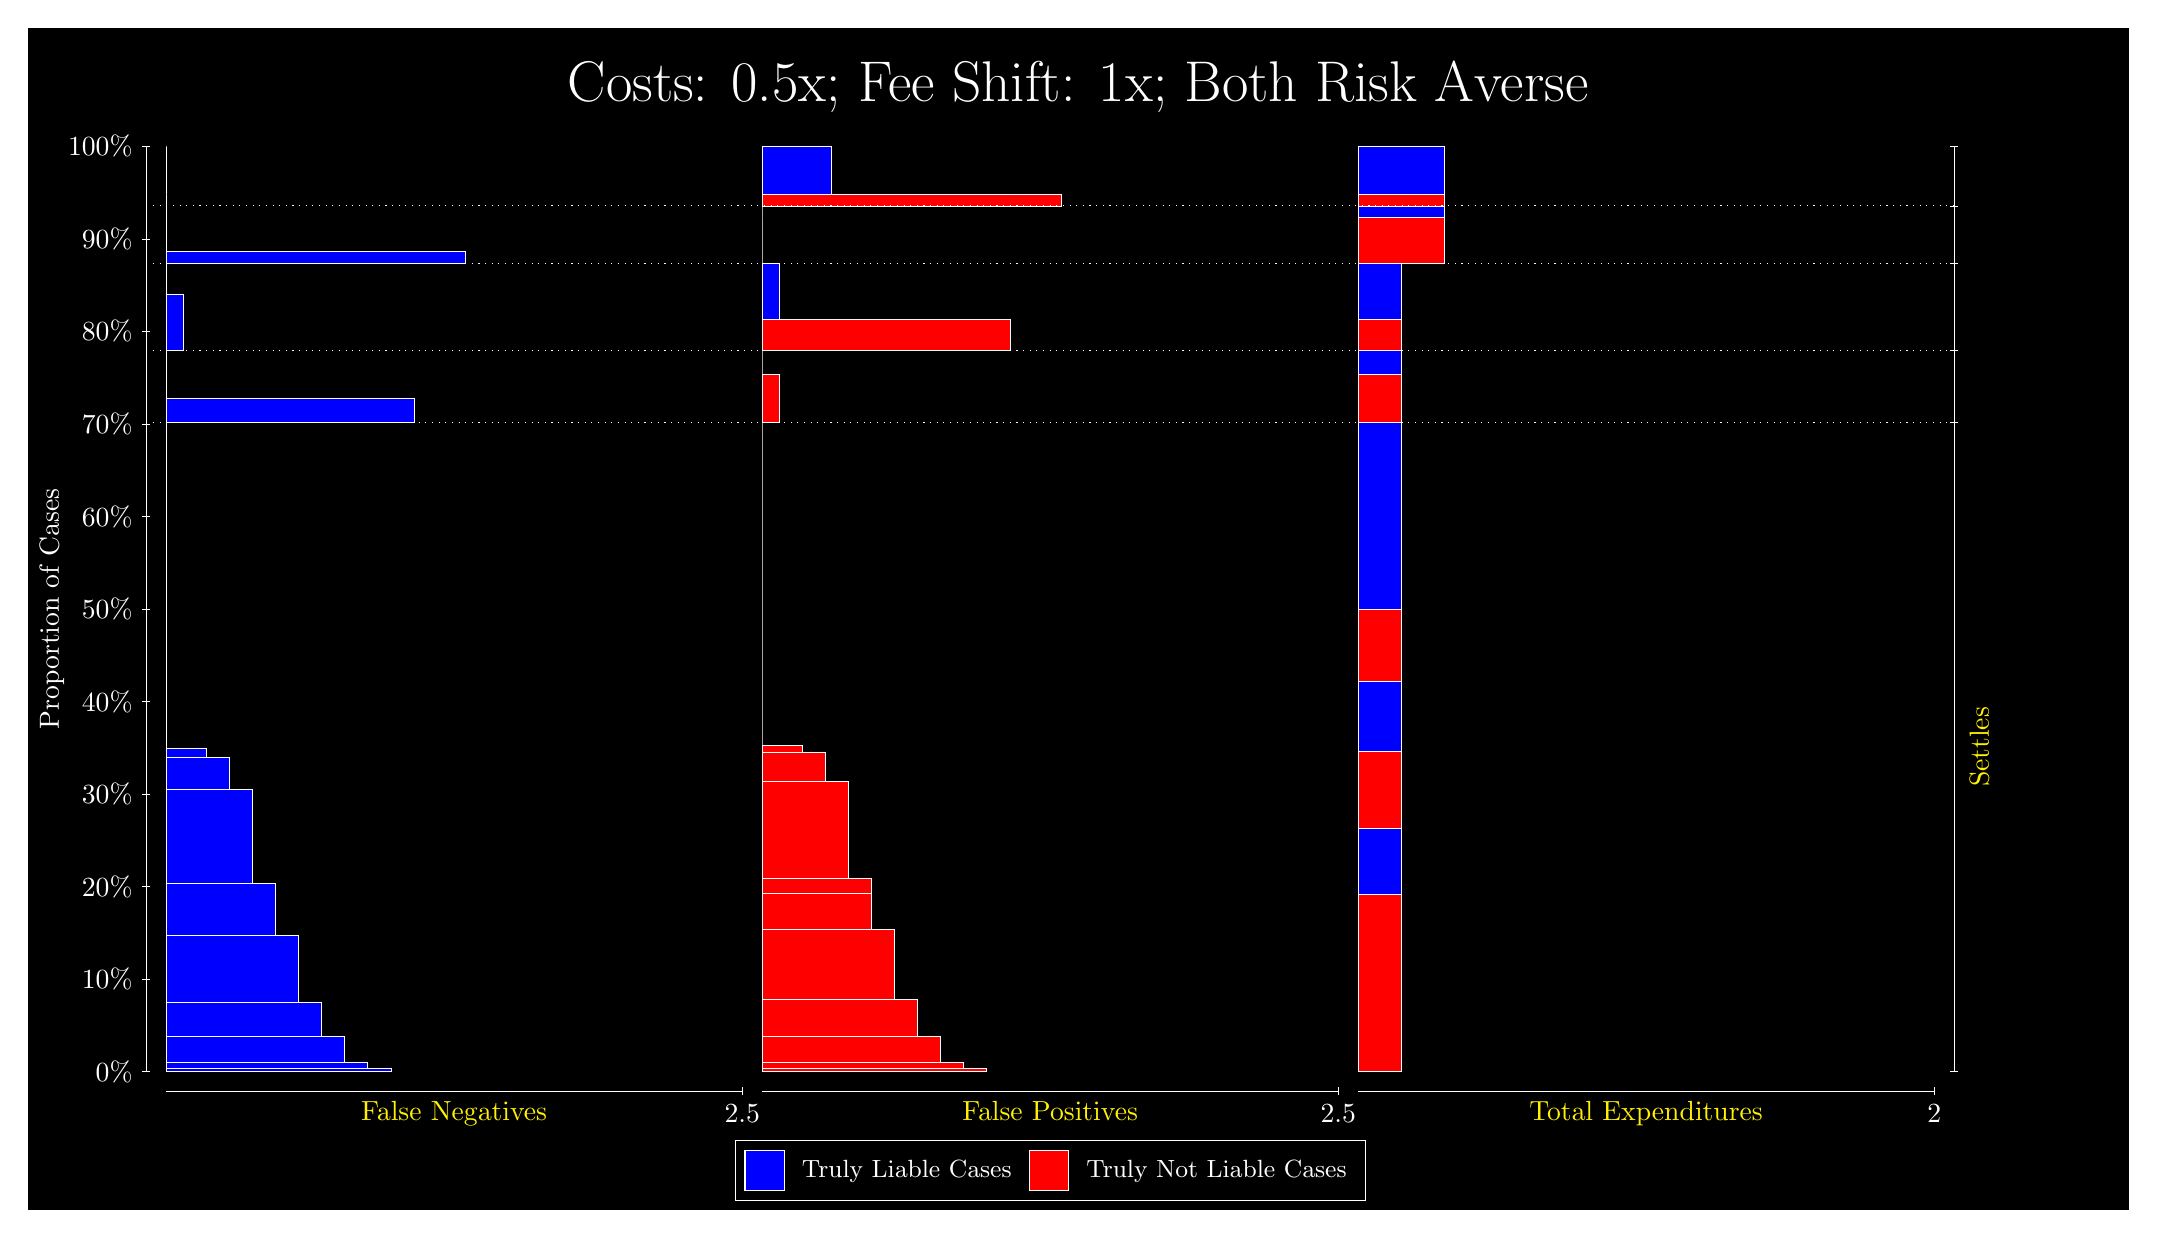
\begin{tikzpicture}
\draw[fill=black] (0,0) rectangle (26.667,15);
\draw[text=white] (0,13.5) rectangle (26.667,15) node[midway] {\huge Costs: 0.5x; Fee Shift: 1x; Both Risk Averse};
\draw[white, very thin] (1.5,1.75) -- (1.5,13.5);
\node[rotate=90, text=white, anchor=center] at (0.3, 7.625) {Proportion of Cases};
\draw[white, very thin] (1.45,1.75) -- (1.55,1.75);
\node[text=white, anchor=east] at (1.45, 1.75) {0\%};
\draw[white, very thin] (1.45,2.925) -- (1.55,2.925);
\node[text=white, anchor=east] at (1.45, 2.925) {10\%};
\draw[white, very thin] (1.45,4.1) -- (1.55,4.1);
\node[text=white, anchor=east] at (1.45, 4.1) {20\%};
\draw[white, very thin] (1.45,5.275) -- (1.55,5.275);
\node[text=white, anchor=east] at (1.45, 5.275) {30\%};
\draw[white, very thin] (1.45,6.45) -- (1.55,6.45);
\node[text=white, anchor=east] at (1.45, 6.45) {40\%};
\draw[white, very thin] (1.45,7.625) -- (1.55,7.625);
\node[text=white, anchor=east] at (1.45, 7.625) {50\%};
\draw[white, very thin] (1.45,8.8) -- (1.55,8.8);
\node[text=white, anchor=east] at (1.45, 8.8) {60\%};
\draw[white, very thin] (1.45,9.975) -- (1.55,9.975);
\node[text=white, anchor=east] at (1.45, 9.975) {70\%};
\draw[white, very thin] (1.45,11.15) -- (1.55,11.15);
\node[text=white, anchor=east] at (1.45, 11.15) {80\%};
\draw[white, very thin] (1.45,12.325) -- (1.55,12.325);
\node[text=white, anchor=east] at (1.45, 12.325) {90\%};
\draw[white, very thin] (1.45,13.5) -- (1.55,13.5);
\node[text=white, anchor=east] at (1.45, 13.5) {100\%};

\draw[white, very thin] (24.457,1.75) -- (24.457,13.5);
\draw[white, very thin] (24.407,1.75) -- (24.507,1.75);
\node[anchor=west] at (24.407, 1.75) {};
\draw[white, very thin] (24.407,9.9964) -- (24.507,9.9964);
\node[anchor=west] at (24.407, 9.9964) {};
\draw[white, very thin] (24.407,10.907) -- (24.507,10.907);
\node[anchor=west] at (24.407, 10.907) {};
\draw[white, very thin] (24.407,12.016) -- (24.507,12.016);
\node[anchor=west] at (24.407, 12.016) {};
\draw[white, very thin] (24.407,12.743) -- (24.507,12.743);
\node[anchor=west] at (24.407, 12.743) {};
\draw[white, very thin] (24.407,13.5) -- (24.507,13.5);
\node[anchor=west] at (24.407, 13.5) {};

\draw[white, very thin, fill=blue] (1.75,1.75) rectangle (4.6044,1.7854);
\draw[white, very thin, fill=blue] (1.75,1.7854) rectangle (4.3116,1.8651);
\draw[white, very thin, fill=blue] (1.75,1.8651) rectangle (4.0188,2.2019);
\draw[white, very thin, fill=blue] (1.75,2.2019) rectangle (3.7261,2.6245);
\draw[white, very thin, fill=blue] (1.75,2.6245) rectangle (3.4333,3.4792);
\draw[white, very thin, fill=blue] (1.75,3.4792) rectangle (3.1406,4.1352);
\draw[white, very thin, fill=blue] (1.75,4.1352) rectangle (2.8478,5.3405);
\draw[white, very thin, fill=blue] (1.75,5.3405) rectangle (2.5551,5.7351);
\draw[white, very thin, fill=blue] (1.75,5.7351) rectangle (2.2623,5.851);
\draw[white, very thin, fill=red] (1.75,5.851) rectangle (1.75,9.9964);
\draw[white, very thin, fill=blue] (1.75,9.9964) rectangle (4.8971,10.298);
\draw[white, very thin, fill=red] (1.75,10.298) rectangle (1.75,10.907);
\draw[white, very thin, fill=blue] (1.75,10.907) rectangle (1.9696,11.623);
\draw[white, very thin, fill=red] (1.75,11.623) rectangle (1.75,12.016);
\draw[white, very thin, fill=blue] (1.75,12.016) rectangle (5.5558,12.161);
\draw[white, very thin, fill=red] (1.75,12.161) rectangle (1.75,12.743);
\draw[white, very thin, fill=red] (1.75,12.743) rectangle (1.75,12.889);
\draw[white, very thin, fill=blue] (1.75,12.889) rectangle (1.75,13.5);
\draw[white, very thin, fill=red] (9.3189,1.75) rectangle (12.173,1.7864);
\draw[white, very thin, fill=red] (9.3189,1.7864) rectangle (11.88,1.8657);
\draw[white, very thin, fill=red] (9.3189,1.8657) rectangle (11.588,2.1941);
\draw[white, very thin, fill=red] (9.3189,2.1941) rectangle (11.295,2.6683);
\draw[white, very thin, fill=red] (9.3189,2.6683) rectangle (11.002,3.5531);
\draw[white, very thin, fill=red] (9.3189,3.5531) rectangle (10.709,4.0114);
\draw[white, very thin, fill=red] (9.3189,4.0114) rectangle (10.709,4.2081);
\draw[white, very thin, fill=red] (9.3189,4.2081) rectangle (10.417,5.4398);
\draw[white, very thin, fill=red] (9.3189,5.4398) rectangle (10.124,5.8036);
\draw[white, very thin, fill=red] (9.3189,5.8036) rectangle (9.8312,5.8954);
\draw[white, very thin, fill=blue] (9.3189,5.8954) rectangle (9.3189,9.9964);
\draw[white, very thin, fill=red] (9.3189,9.9964) rectangle (9.5384,10.606);
\draw[white, very thin, fill=blue] (9.3189,10.606) rectangle (9.3189,10.907);
\draw[white, very thin, fill=red] (9.3189,10.907) rectangle (12.466,11.3);
\draw[white, very thin, fill=blue] (9.3189,11.3) rectangle (9.5384,12.016);
\draw[white, very thin, fill=red] (9.3189,12.016) rectangle (9.3189,12.597);
\draw[white, very thin, fill=blue] (9.3189,12.597) rectangle (9.3189,12.743);
\draw[white, very thin, fill=red] (9.3189,12.743) rectangle (13.125,12.889);
\draw[white, very thin, fill=blue] (9.3189,12.889) rectangle (10.197,13.5);
\draw[white, very thin, fill=red] (16.888,1.75) rectangle (17.437,4.0005);
\draw[white, very thin, fill=blue] (16.888,4.0005) rectangle (17.437,4.8396);
\draw[white, very thin, fill=red] (16.888,4.8396) rectangle (17.437,5.8163);
\draw[white, very thin, fill=blue] (16.888,5.8163) rectangle (17.437,6.7064);
\draw[white, very thin, fill=red] (16.888,6.7064) rectangle (17.437,7.6247);
\draw[white, very thin, fill=blue] (16.888,7.6247) rectangle (17.437,9.9964);
\draw[white, very thin, fill=red] (16.888,9.9964) rectangle (17.437,10.606);
\draw[white, very thin, fill=blue] (16.888,10.606) rectangle (17.437,10.907);
\draw[white, very thin, fill=red] (16.888,10.907) rectangle (17.437,11.3);
\draw[white, very thin, fill=blue] (16.888,11.3) rectangle (17.437,12.016);
\draw[white, very thin, fill=red] (16.888,12.016) rectangle (17.986,12.597);
\draw[white, very thin, fill=blue] (16.888,12.597) rectangle (17.986,12.743);
\draw[white, very thin, fill=red] (16.888,12.743) rectangle (17.986,12.889);
\draw[white, very thin, fill=blue] (16.888,12.889) rectangle (17.986,13.5);
\draw[white, dotted] (1.5,9.9964) -- (24.457,9.9964);
\draw[white, dotted] (1.5,10.907) -- (24.457,10.907);
\draw[white, dotted] (1.5,12.016) -- (24.457,12.016);
\draw[white, dotted] (1.5,12.743) -- (24.457,12.743);
\draw[white, very thin] (1.75,1.5) -- (9.0689,1.5);
\node[text=yellow, anchor=north] at (5.4094, 1.5) {False Negatives};
\draw[white, very thin] (9.0689,1.45) -- (9.0689,1.55);
\node[text=white, anchor=north] at (9.0689, 1.45) {2.5};

\draw[white, very thin] (9.3189,1.5) -- (16.638,1.5);
\node[text=yellow, anchor=north] at (12.978, 1.5) {False Positives};
\draw[white, very thin] (16.638,1.45) -- (16.638,1.55);
\node[text=white, anchor=north] at (16.638, 1.45) {2.5};

\draw[white, very thin] (16.888,1.5) -- (24.207,1.5);
\node[text=yellow, anchor=north] at (20.547, 1.5) {Total Expenditures};
\draw[white, very thin] (24.207,1.45) -- (24.207,1.55);
\node[text=white, anchor=north] at (24.207, 1.45) {2};

\node[text=yellow, centered, rotate=90] at (24.777, 5.8732) {Settles};





\draw (12.978300999999998,1.5) node[draw=none] (baseCoordinate) {};
\begin{scope}[align=center]
        \matrix[scale=0.5, draw=white, below=0.5cm of baseCoordinate, nodes={draw}, column sep=0.1cm]{
            \node[rectangle, draw, minimum width=0.5cm, minimum height=0.5cm, fill=blue] {}; &
            \node[draw=none, font=\small, text=white] (B) {Truly Liable Cases}; &
            \node[rectangle, draw, minimum width=0.5cm, minimum height=0.5cm, fill=red] {}; &
            \node[draw=none, font=\small, text=white] (B) {Truly Not Liable Cases}; \\
            };
\end{scope}

\end{tikzpicture}
\end{document}